\documentclass{article}
\usepackage{amsmath} % Required for math symbols and formatting
\usepackage{tikz}    % Required for TikZ package

\begin{document}
\noindent
Integrals for Area between a curve:
\[
A = \int (top - bottom) \, dx
\]
\[
Washers: V = \int (\pi R^2 - \pi r^2) \, dx
\] 
\[
Shells: V = \int (2 \pi (radius)(top - bottom) ) \, dx
\] 
\text{Integral for Work}:
\[
W = \int (Force)(Distance) \, dx
\] 
\text{Integral for Averages}:
\[
F_{\text{av}}: \frac{1}{b-a} = \int_{a}^{b} f(x) \, dx
\] 
Integration By Parts: 
\[
IBP: \int u \, dv = \int v \, du
\] 
Improper Integrals:
\[
\int_{a}^{\infty} \frac{1}{x^p} \, dx = 
\begin{cases}
\text{Converges if } p > 1 \\
\text{Diverges if } p \leq 1
\end{cases}
\]
\[
\int_{0}^{a} \frac{1}{x^p} \, dx = 
\begin{cases}
\text{Converges if } p < 1 \\
\text{Diverges if } p \geq 1
\end{cases}
\]
$\text{constant} < \ln(x) < \text{poly} < \text{exponential}$

Trig Sub:

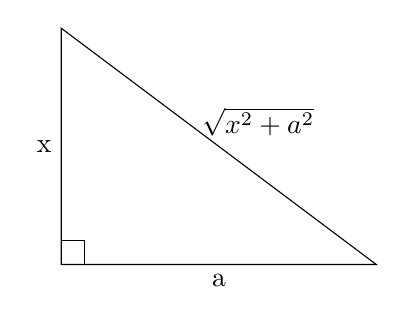
\begin{tikzpicture}[xshift=0cm] % Adjust the xshift for the first triangle
% Draw the first triangle
\draw (0,0) -- (4,0) -- (0,3) -- cycle;
% Label the sides
\node[left] at (0,1.5) {x};
\node[below] at (2,0) {a};
% Label the right angle
\draw (0.3,0) -- (0.3,0.3) -- (0,0.3);
% Label the hypotenuse with a square root expression
\node[above] at (2.5,1.5) {$\sqrt{x^2+a^2}$};
\end{tikzpicture}
% Adjust the xshift for the second triangle
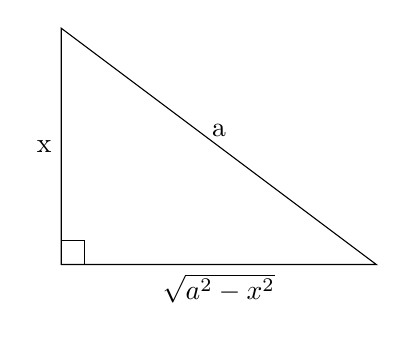
\begin{tikzpicture}[xshift=2cm] % Adjust the xshift for the second triangle
% Draw the second triangle
\draw (0,0) -- (4,0) -- (0,3) -- cycle;
% Label the sides
\node[left] at (0,1.5) {x};
\node[below] at (2,0) {$\sqrt{a^2-x^2}$};
\node[above] at (2,1.5) {a};
% Label the right angle
\draw (0.3,0) -- (0.3,0.3) -- (0,0.3);
\end{tikzpicture}%
% Adjust the xshift for the third triangle
\begin{tikzpicture}[xshift=4cm] % Adjust the xshift for the third triangle
% Draw the third triangle
\draw (0,0) -- (4,0) -- (0,3) -- cycle;
% Label the sides
\node[left] at (0,1.5) {$\sqrt{x^2-a^2}$};
\node[below] at (2,0) {a};
\node[above] at (2,1.5) {x};
% Label the right angle
\draw (0.3,0) -- (0.3,0.3) -- (0,0.3);
\end{tikzpicture}%

\hspace{1cm} 1.)\enskip $x = a\tan(\theta)$ \quad \hspace{1.25cm} 2.)\enskip $x = a\sin(\theta)$ \quad \hspace{1cm} 3.)\enskip $x = a\sec(\theta)$

\hspace{1cm} 1.)\enskip $x = a\sec^2(\theta) d(\theta)$ \phantom{2.)\enskip} 2.)\enskip $x = a\cos(\theta) d(\theta)$ \phantom{3.)\enskip} 3.)\enskip $x = a\sec(\theta)\tan(\theta) d(\theta)$


\end{document}
